\documentclass[11pt]{article}
\usepackage[a4paper, total={6in, 12in}]{geometry}
\usepackage{graphicx}
\usepackage{amsmath,amsfonts,amssymb}
\usepackage{listings}
\usepackage{booktabs}
\usepackage[T1]{fontenc}
\usepackage{color}
\usepackage{minted}
\usepackage[colorlinks=true, linkcolor=blue, urlcolor=blue, citecolor=blue,
  pdfborder={0 0 255}]{hyperref}
\usepackage{colortbl}
\usepackage{url}
\usepackage{xcolor}
\usepackage{caption}
\usepackage{subcaption}
\usepackage{dirtytalk}
\usepackage[semicolon, round]{natbib}
\usepackage[ruled]{algorithm2e}
\usepackage{multirow}
\usepackage{setspace}
\usepackage{placeins}
\captionsetup[table]{skip=10pt}
\renewcommand{\vec}[1]{\mathbf{#1}}
\SetKwComment{Comment}{$\triangleright$\ }{}
% \hypersetup{%
% 	colorlinks=true,
% 	linkcolor=blue,
% 	linkbordercolor={0 0 1}
% }

% \renewcommand\lstlistingname{Algorithm}
% \renewcommand\lstlistlistingname{Algorithms}
% \def\lstlistingautorefname{Alg.}

% \lstdefinestyle{Python}{
% 	language        = Python,
% 	frame           = lines,
% 	basicstyle      = \footnotesize,
% 	keywordstyle    = \color{blue},
% 	stringstyle     = \color{green},
% 	commentstyle    = \color{red}\ttfamily
% }

\setlength{\parindent}{0.0in}
\setlength{\parskip}{0.02in}

\newcommand{\argmin}{\mathop{\mathrm{argmin}}}
\newcommand{\argmax}{\mathop{\mathrm{argmax}}}
\newcommand{\minimize}{\mathop{\mathrm{minimize}}}
\newcommand{\maximize}{\mathop{\mathrm{maximize}}}
\newcommand{\st}{\mathop{\mathrm{subject\,\,to}}}
\newcommand{\dist}{\mathop{\mathrm{dist}}}
\newcommand{\norm}[1]{\left\lVert#1\right\rVert}
\renewcommand{\vec}[1]{\mathbf{#1}}

\DeclareCaptionType{codelisting}[Listing][List of mytype]
\newenvironment{codeblock}{\captionsetup{type=codelisting}}{}

\def\R{\mathbb{R}}
\def\E{\mathbb{E}}
\def\P{\mathbb{P}}
\def\S{\mathbb{S}}
\def\Cov{\mathrm{Cov}}
\def\Var{\mathrm{Var}}
\def\half{\frac{1}{2}}
\def\quat{\frac{1}{4}}
\def\sign{\mathrm{sign}}
\def\supp{\mathrm{supp}}
\def\th{\mathrm{th}}
\def\tr{\mathrm{tr}}
\def\dim{\mathrm{dim}}
\def\dom{\mathrm{dom}}

\title{EE2003 Assignment 1 \vspace{-1em}}
\author{Niranjan A. Kartha, EE21B095\vspace{-3em}}
\date{}

\begin{document}
\maketitle
\section*{P4. Question}
Write a program to Compare Two Words (ie, two 4 digit hexadecimal numbers) and display the result in \texttt{RESULT}. If the Words are equal \texttt{RESULT} should be set as zero, else set as one.

\subsection*{Logic used}
Two numbers \texttt{X} and \texttt{Y} are to be compared. This is done by first loading \texttt{X} in the accumulator, taking its two's complement ($\bar{\texttt{X}} + 1$), then adding \texttt{Y} to it. This gives us the value of $\texttt{Y} - \texttt{X}$ in the accumulator. Now, if $\texttt{Y} - \texttt{X}$ is non-zero, we load the value of \texttt{1} into the accumulator, else we leave it as-is. Then, we store the value of the accumlator in \texttt{RESULT}.

\subsection*{Program}

\begin{codeblock}
\inputminted[breaklines,
 mathescape,
 linenos,
 numbersep=5pt,
 frame=single,
 numbersep=5pt,
 xleftmargin=0pt]{asm}{program.s}
\end{codeblock}

\subsection*{Inputs}
when inputs are not equal:
\begin{codeblock}
\inputminted[breaklines,
 mathescape,
 linenos,
 numbersep=5pt,
 frame=single,
 numbersep=5pt,
 xleftmargin=0pt]{asm}{inputs1.s}
\end{codeblock}

when inputs are equal:
\begin{codeblock}
\inputminted[breaklines,
 mathescape,
 linenos,
 numbersep=5pt,
 frame=single,
 numbersep=5pt,
 xleftmargin=0pt]{asm}{inputs2.s}
\end{codeblock}

\subsection*{Outputs}
\begin{figure}[H]
\begin{subfigure}{.5\textwidth}
  \centering
  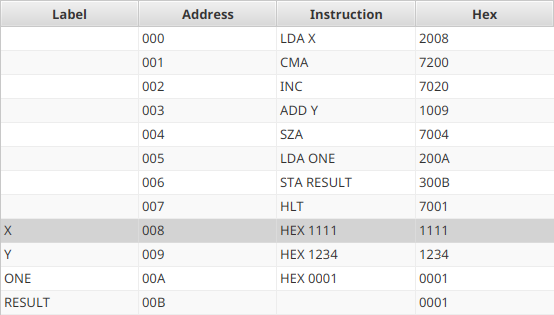
\includegraphics[width=\linewidth]{out-neq.png}
  \caption*{with non-equal inputs}
\end{subfigure}
\begin{subfigure}{.5\textwidth}
  \centering
  % include second image
  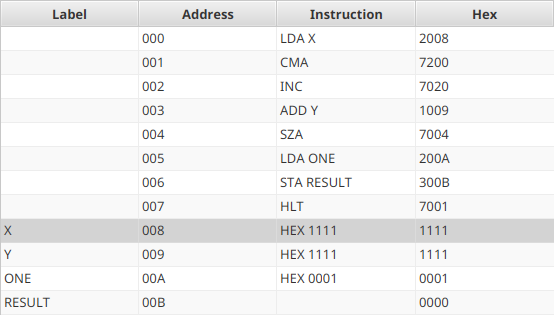
\includegraphics[width=\linewidth]{out-eq.png}
  \caption*{with equal inputs}
\end{subfigure}
\end{figure}

\end{document}
